\chapter{Quantum Dot Results}

Here we present supplementary data that completes the results presented in 
\autoref{ch:quantum_dots} on quantum dot simulations in time. In this appendix we 
show how the time-dependent coupled cluster method 
converges for an increasing basis. These simulations are done for quantum dots in both
one and two dimensions.
Additionally, we provide the results from simulations constructed to show the response 
of quantum dots subjected to oscillating fields of different frequencies.
Lastly, we show how a quantum dot in two
dimensions, subject to a magnetic field, leads to a splitting in the dipole spectrum 
of the system.

\vfill
\pagebreak

\section{One Dimension}
\label{app:1d_qd}

The simulations presented here have been conducted with the Time-Dependent Coupled 
Cluster Singled Doubles (TDCCSD) method.

\subsection*{Four electrons}

\begin{figure}[h]
    \centering
    \makebox[\textwidth][c]{
    \begin{minipage}{0.6\textwidth}
        \centering
        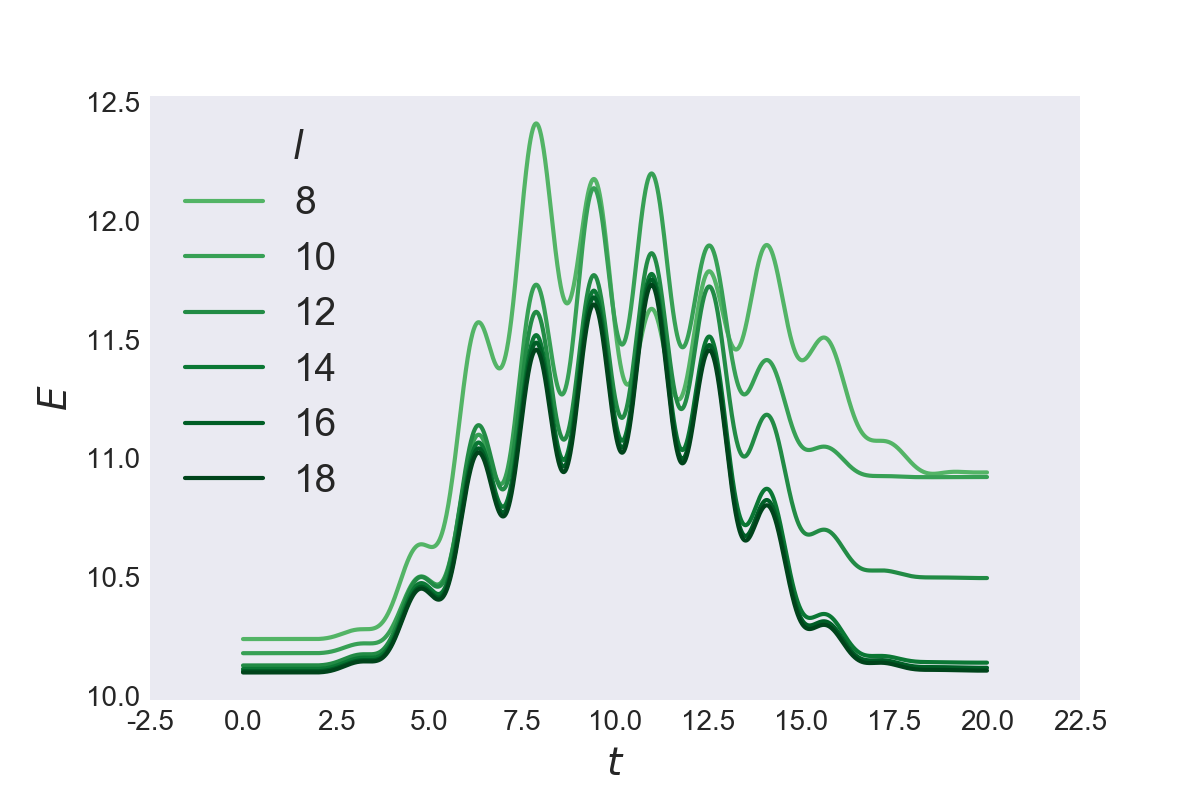
\includegraphics[width=\textwidth]{results/figures/1D/n=4energy.png}
    \end{minipage}\hfill 
    \begin{minipage}{0.6\textwidth}
        \centering 
        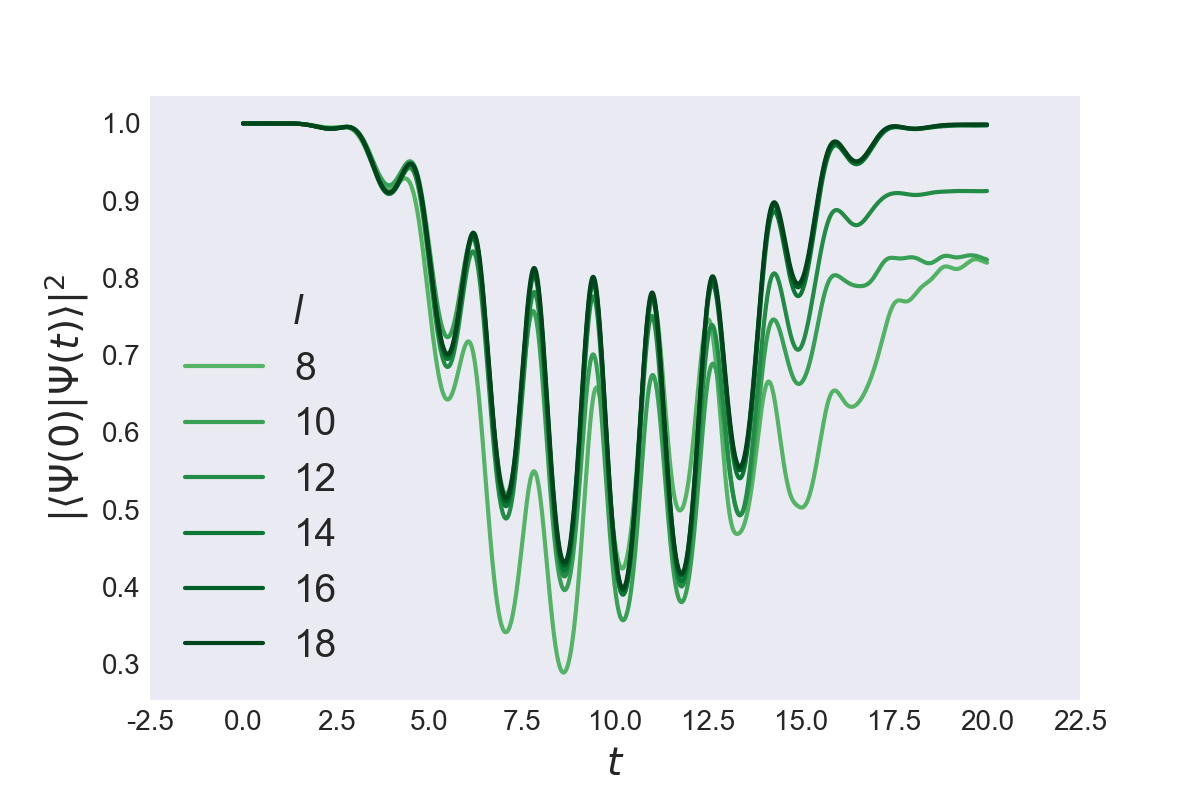
\includegraphics[width=\textwidth]{results/figures/1D/n=4overlap.png}
    \end{minipage}
    }
    \caption{Time-dependent energy (left) and ground state probability (right)
        of a one-dimensional harmonic oscillator with $\Omega=1 \text{ a.u.}$
        and $n=4$ electrons under the influence of a oscillating electric field 
        of frequency $\omega = 2 \Omega = 2 \text{ a.u.}$ and field strength
        $E_\text{max}=1 \text{ a.u.}$,
        for different number of spin-orbitals $l=\{8,10,12,14,16,18\}$.
    }
    \label{fig:1d_n4_qd}
\end{figure}

\begin{figure}[!h]
    \centering
    \makebox[\textwidth][c]{
    \begin{minipage}{0.6\textwidth}
        \centering
        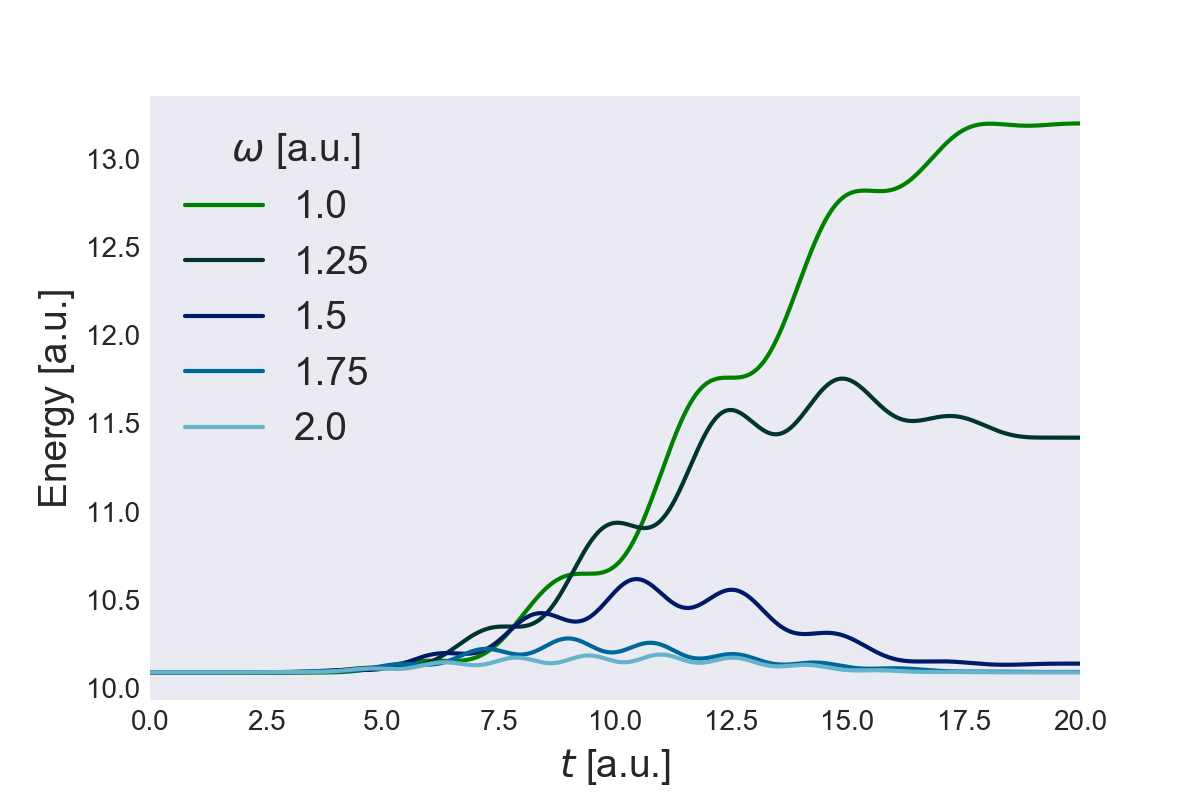
\includegraphics[width=\textwidth]{results/figures/1D/n4_resonance_energy.png}
    \end{minipage}\hfill 
    \begin{minipage}{0.6\textwidth}
        \centering 
        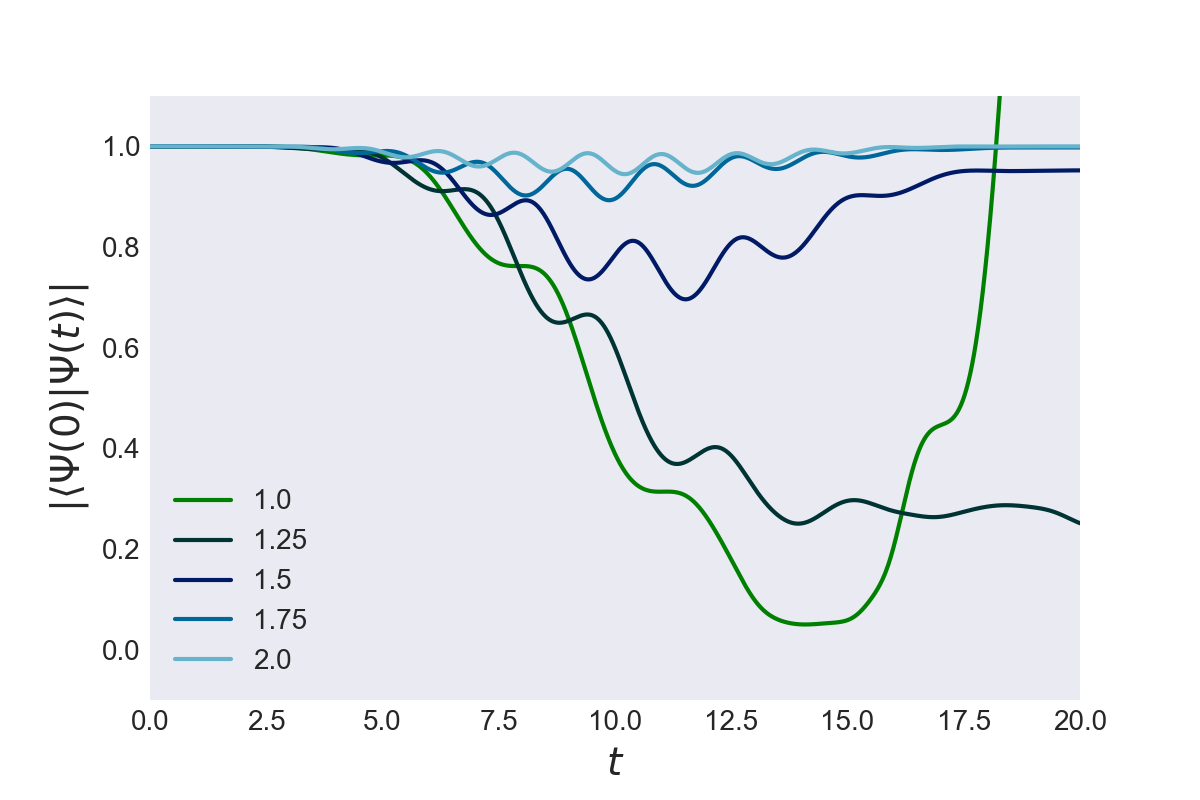
\includegraphics[width=\textwidth]{results/figures/1D/n4_resonance_overlap.png}
    \end{minipage}
    }
    \caption{Time-dependent energy (left) and ground state probability (right)
        of a one-dimensional harmonic oscillator with $\Omega=1 \text{ a.u.}$
        and $n=4$ electrons under the influence of a oscillating electric field 
        of different frequencies $\omega\in\{1.0, 1.25, 1.5, 1.75, 2.0\}$ in 
        atomic units with maximum field strength $E_\text{max}=0.25 \text{ a.u.}$
        and $l=30$ spin-orbitals.
    }
    \label{fig:1d_n4_qd_resonance}
\end{figure}

\vfill
\pagebreak

\subsection*{Six electrons}

\begin{figure}[!h]
    \centering
    \makebox[\textwidth][c]{
    \begin{minipage}{0.6\textwidth}
        \centering
        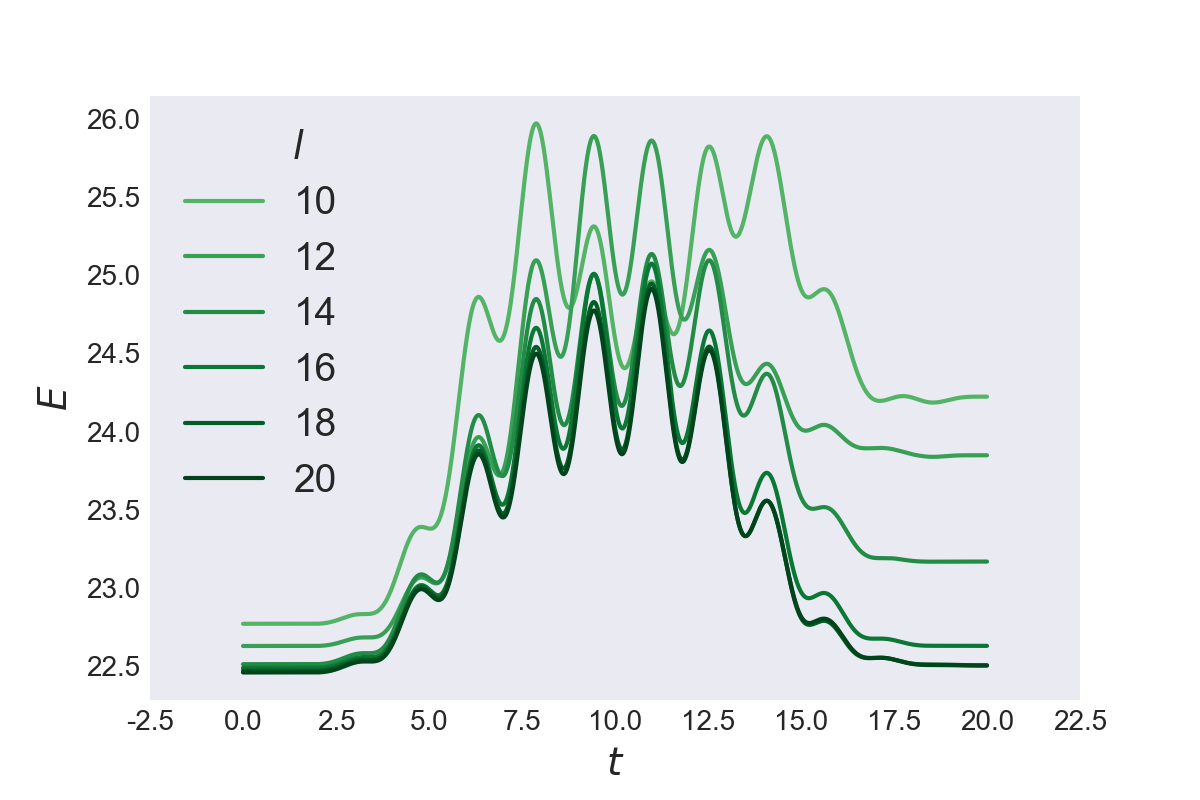
\includegraphics[width=\textwidth]{results/figures/1D/n=6energy.png}
    \end{minipage}\hfill 
    \begin{minipage}{0.6\textwidth}
        \centering 
        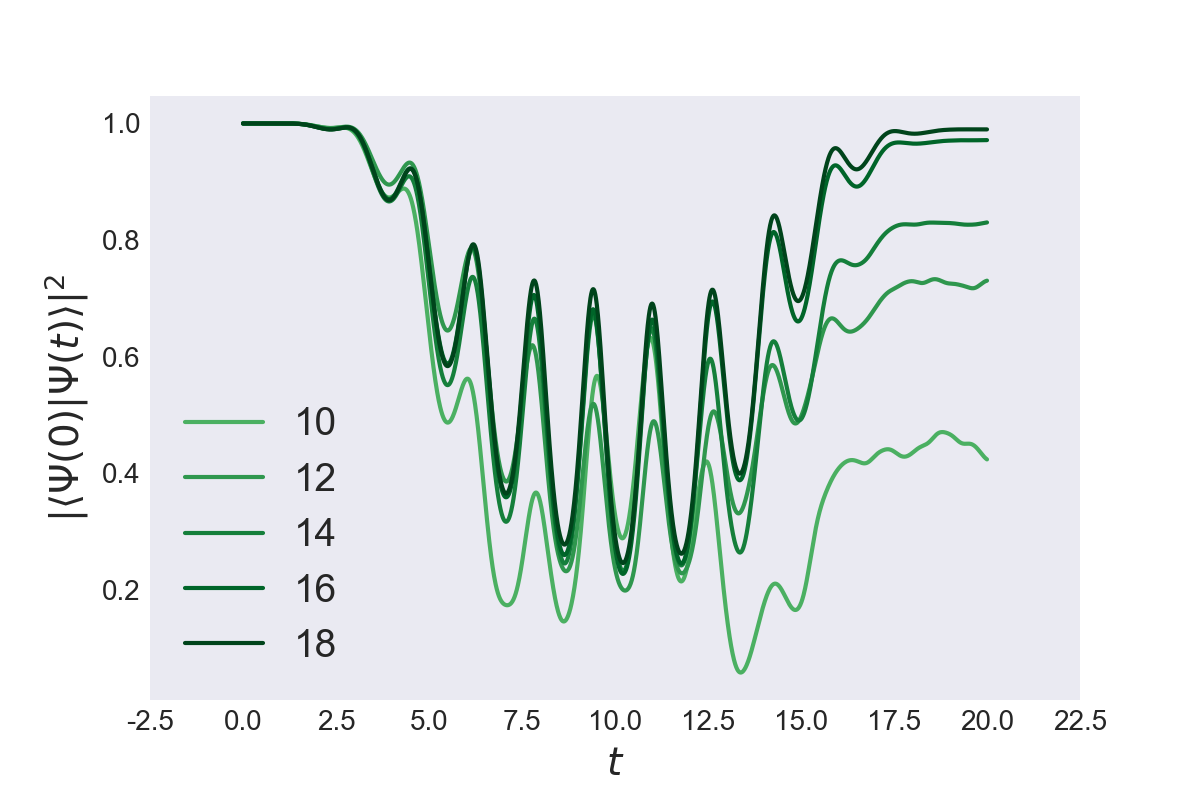
\includegraphics[width=\textwidth]{results/figures/1D/n=6overlap.png}
    \end{minipage}
    }
    \caption{Time-dependent energy (left) and ground state probability (right)
        of a one-dimensional harmonic oscillator with $\Omega=1 \text{ a.u.}$
        and $n=6$ electrons under the influence of a oscillating electric field 
        of frequency $\omega = 2 \Omega = 2 \text{ a.u.}$ and field strength
        $E_\text{max}=1 \text{ a.u.}$,
        for different number of spin-orbitals $l=\{10,12,14,16,18,20\}$.
    }
    \label{fig:1d_n6_qd}
\end{figure}

\begin{figure}[!h]
    \centering
    \makebox[\textwidth][c]{
    \begin{minipage}{0.6\textwidth}
        \centering
        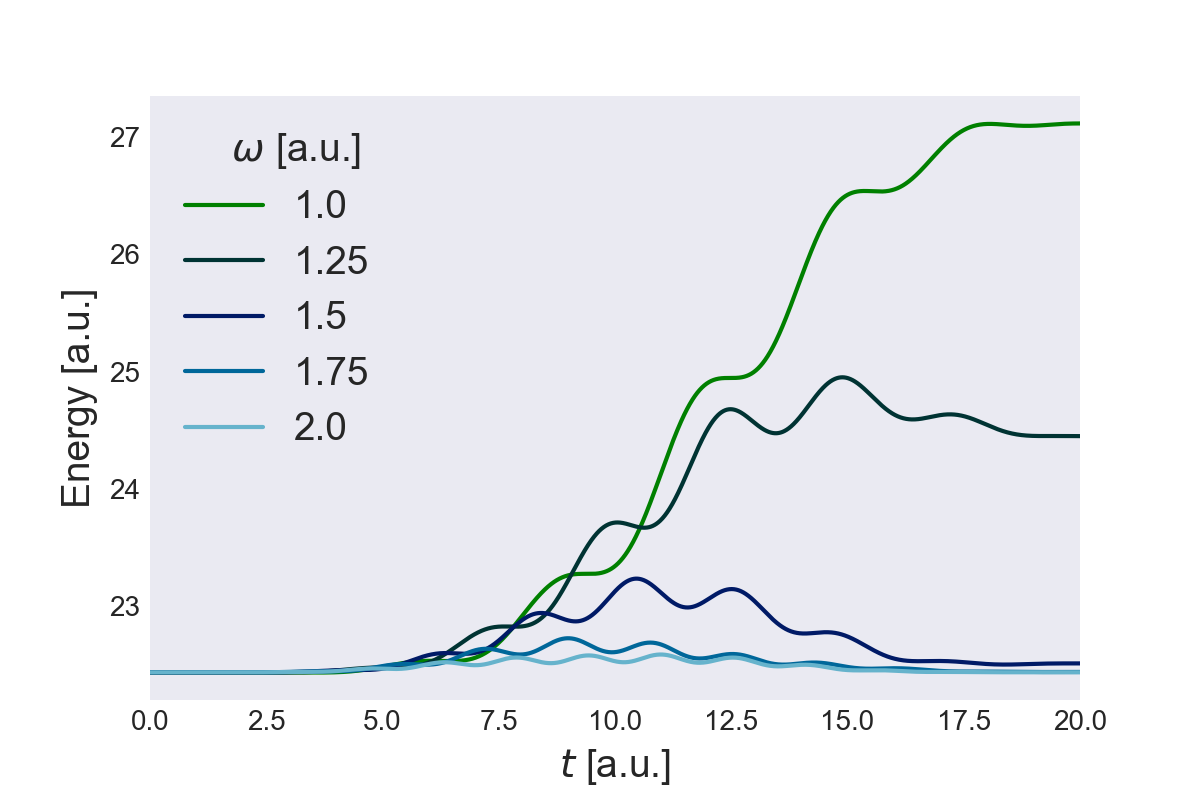
\includegraphics[width=\textwidth]{results/figures/1D/n6_resonance_energy.png}
    \end{minipage}\hfill 
    \begin{minipage}{0.6\textwidth}
        \centering 
        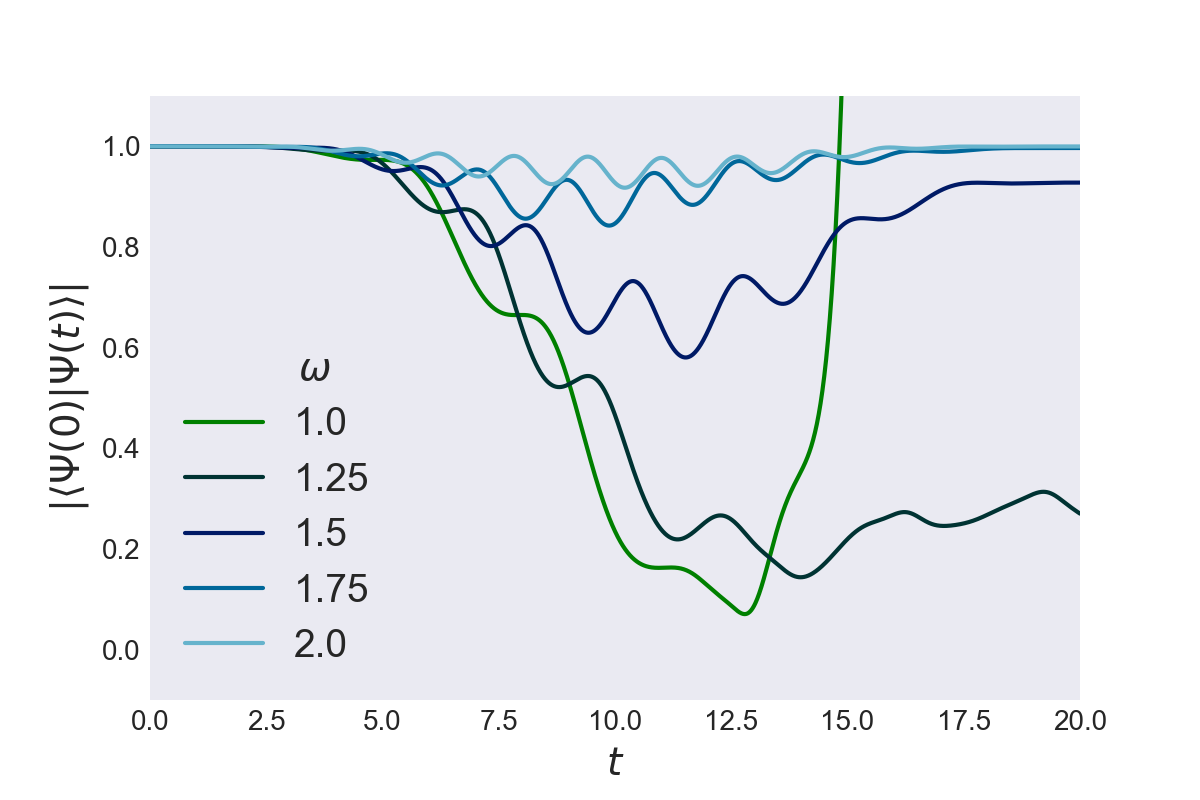
\includegraphics[width=\textwidth]{results/figures/1D/n6_resonance_overlap.png}
    \end{minipage}
    }
    \caption{Time-dependent energy (left) and ground state probability (right)
        of a one-dimensional harmonic oscillator with $\Omega=1 \text{ a.u.}$
        and $n=6$ electrons under the influence of a oscillating electric field 
        of different frequencies $\omega\in\{1.0, 1.25, 1.5, 1.75, 2.0\}$ in atomic units
        with maximum field strength $E_\text{max}=0.25 \text{ a.u.}$ and $l=30$ 
        spin-orbitals.
    }
    \label{fig:1d_n6_qd_resonance}
\end{figure}

\vfill
\pagebreak

\subsection*{Eight electrons}

\begin{figure}[!h]
    \centering
    \makebox[\textwidth][c]{
    \begin{minipage}{0.6\textwidth}
        \centering
        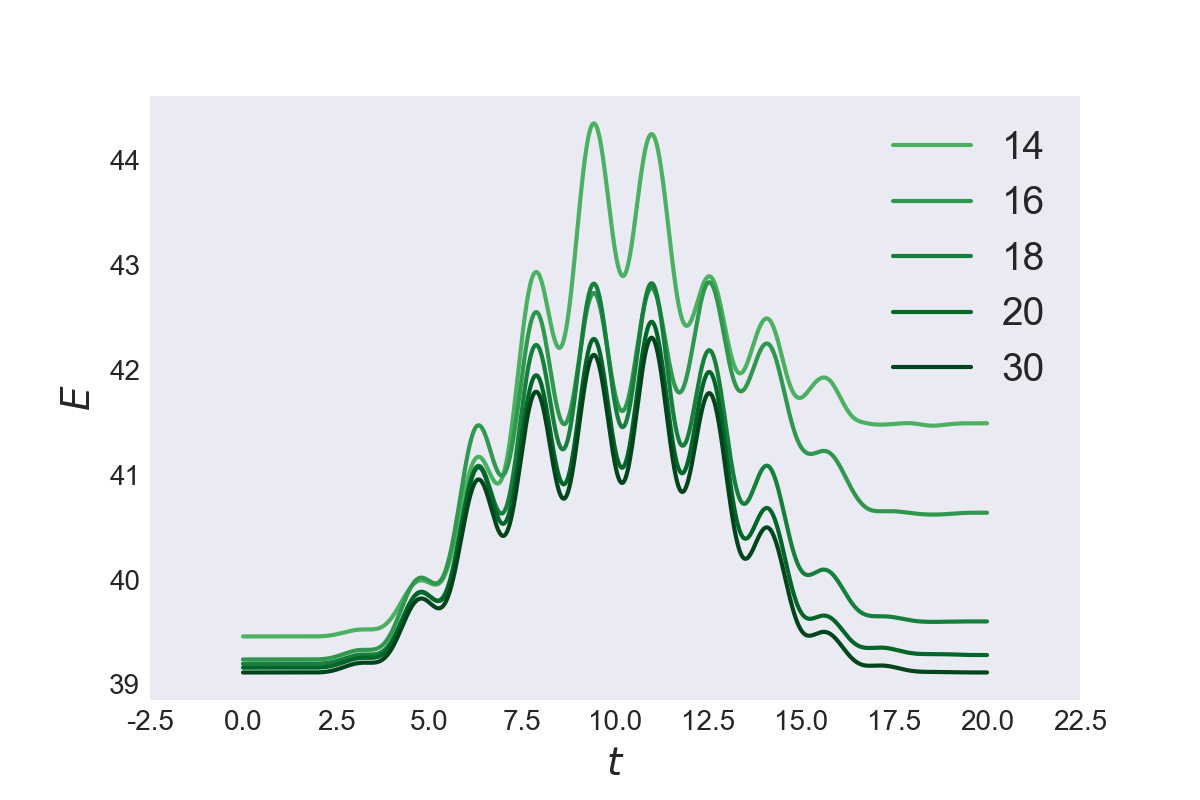
\includegraphics[width=\textwidth]{results/figures/1D/n=8energy.png}
    \end{minipage}\hfill 
    \begin{minipage}{0.6\textwidth}
        \centering 
        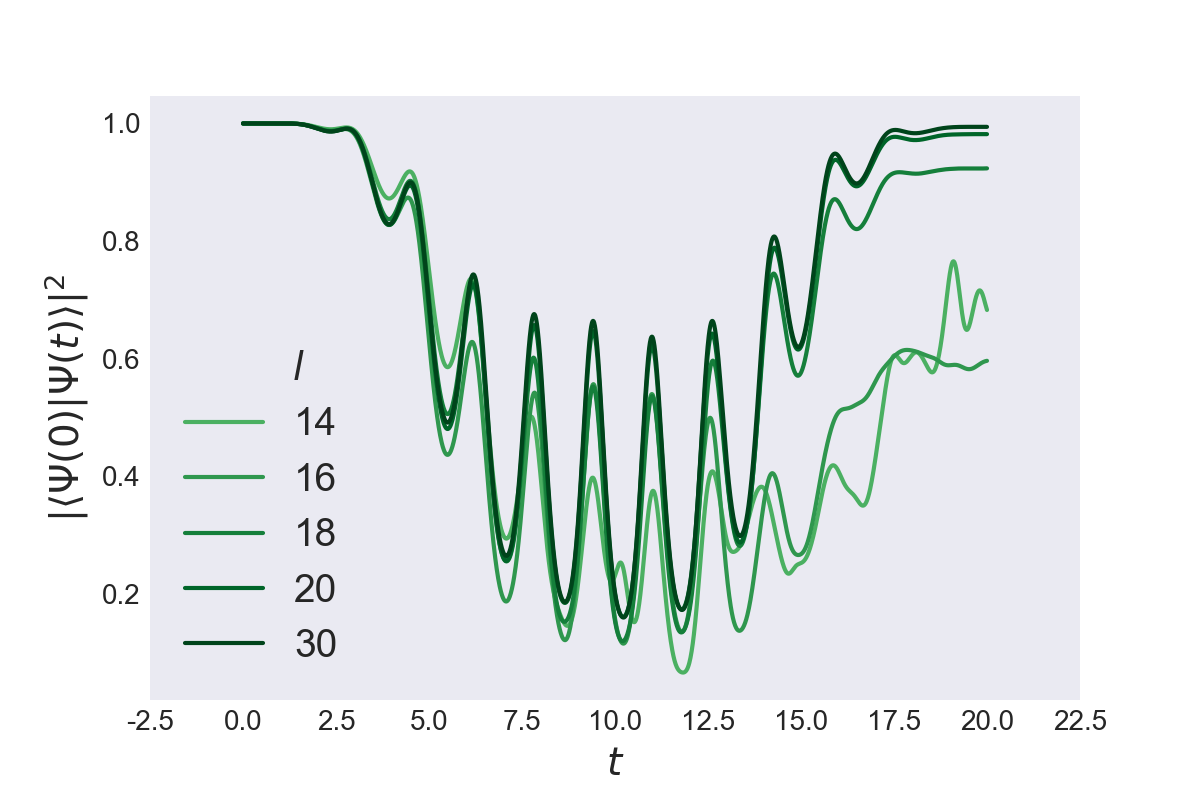
\includegraphics[width=\textwidth]{results/figures/1D/n=8overlap.png}
    \end{minipage}
    }
    \caption{Time-dependent energy (left) and ground state probability (right)
        of a one-dimensional harmonic oscillator with $\Omega=1 \text{ a.u.}$
        and $n=8$ electrons under the influence of a oscillating electric field 
        of frequency $\omega = 2 \Omega = 2 \text{ a.u.}$ and field strength
        $E_\text{max}=1 \text{ a.u.}$,
        for different number of spin-orbitals $l=\{14,16,18,20,30\}$.
    }
    \label{fig:1d_n8_qd}
\end{figure}

\begin{figure}[!h]
    \centering
    \makebox[\textwidth][c]{
    \begin{minipage}{0.6\textwidth}
        \centering
        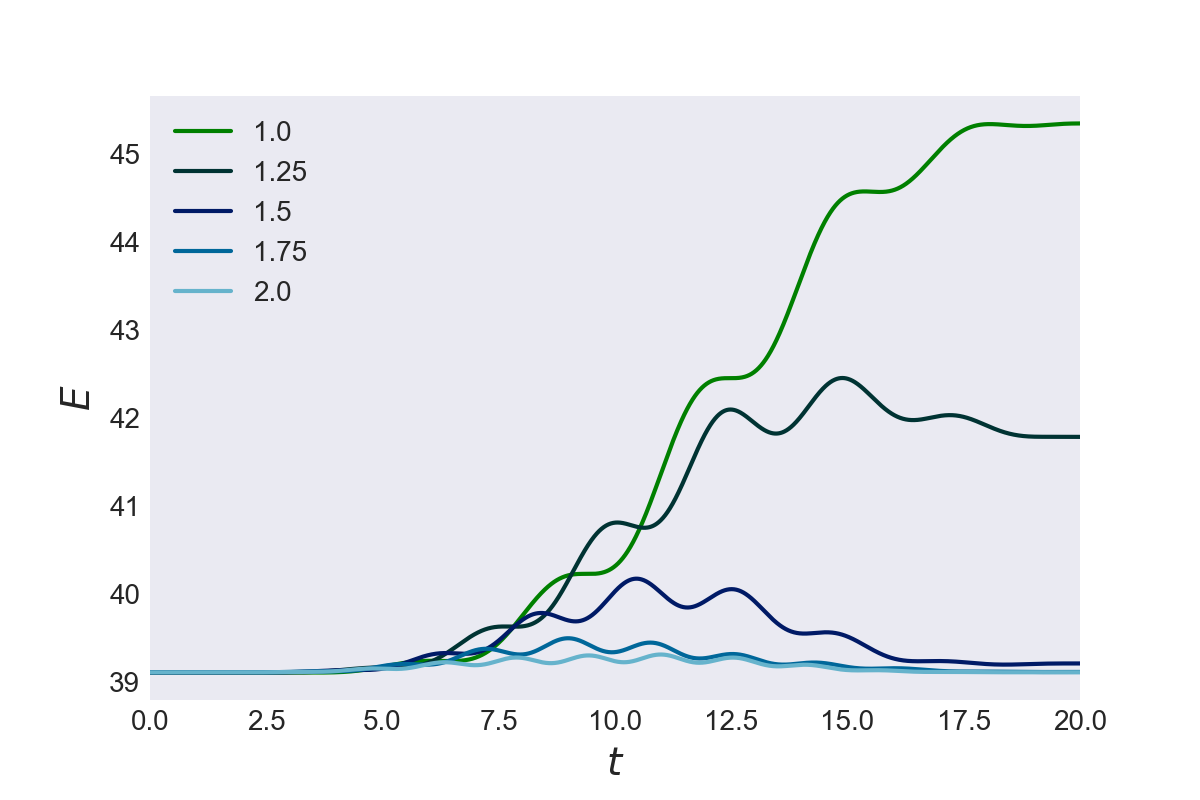
\includegraphics[width=\textwidth]{results/figures/1D/n8_resonance_energy.png}
    \end{minipage}\hfill 
    \begin{minipage}{0.6\textwidth}
        \centering 
        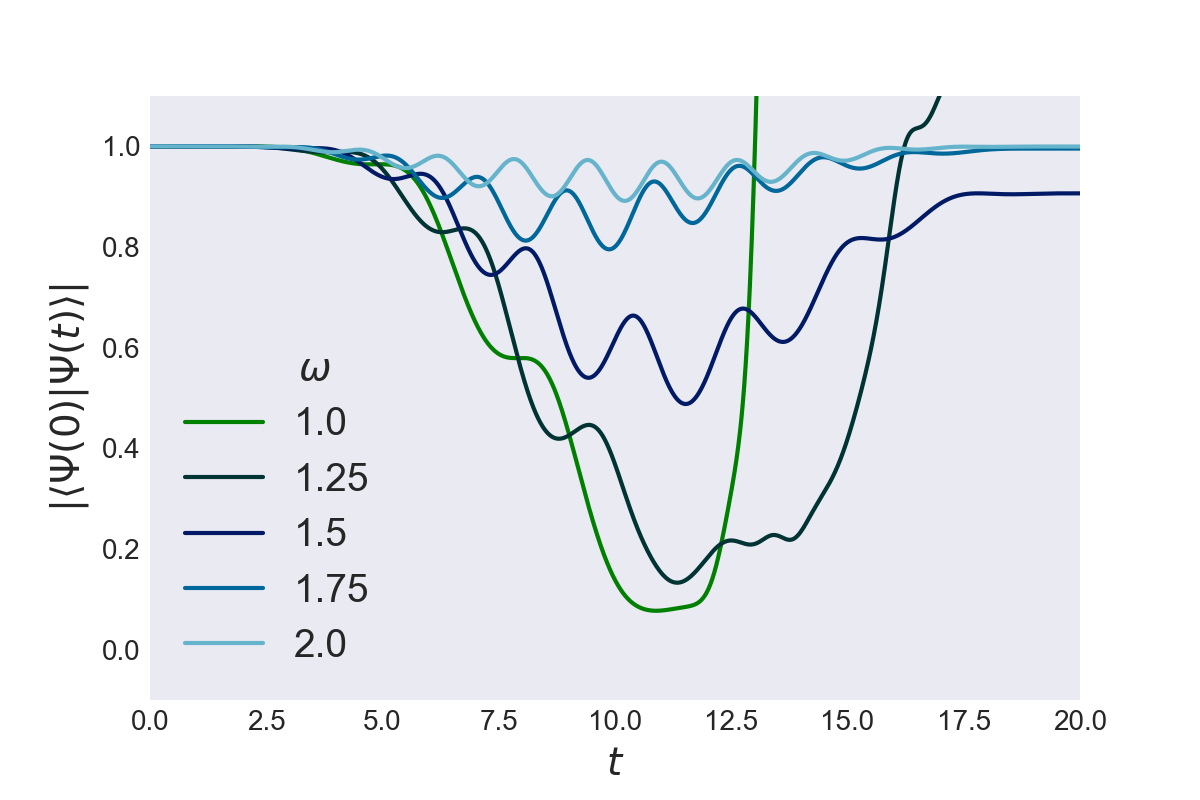
\includegraphics[width=\textwidth]{results/figures/1D/n8_resonance_overlap.png}
    \end{minipage}
    }
    \caption{Time-dependent energy (left) and ground state probability (right)
        of a one-dimensional harmonic oscillator with $\Omega=1 \text{ a.u.}$
        and $n=8$ electrons under the influence of a oscillating electric field 
        of different frequencies $\omega\in\{1.0, 1.25, 1.5, 1.75, 2.0\}$ in atomic 
        orbitals with 
        maximum field strength $E_\text{max}=0.25 \text{ a.u.}$ and $l=36$ 
        spin-orbitals.
    }
    \label{fig:1d_n8_qd_resonance}
\end{figure}

\vfill
\pagebreak

\subsection*{Ten electrons}

\begin{figure}[!h]
    \centering
    \makebox[\textwidth][c]{
    \begin{minipage}{0.6\textwidth}
        \centering
        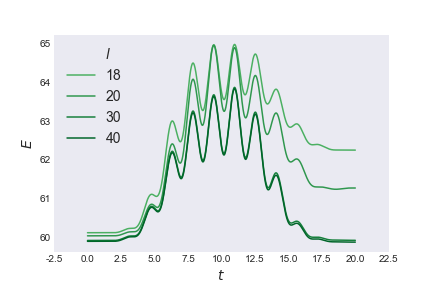
\includegraphics[width=\textwidth]{results/figures/1D/n=10energy.png}
    \end{minipage}\hfill 
    \begin{minipage}{0.6\textwidth}
        \centering 
        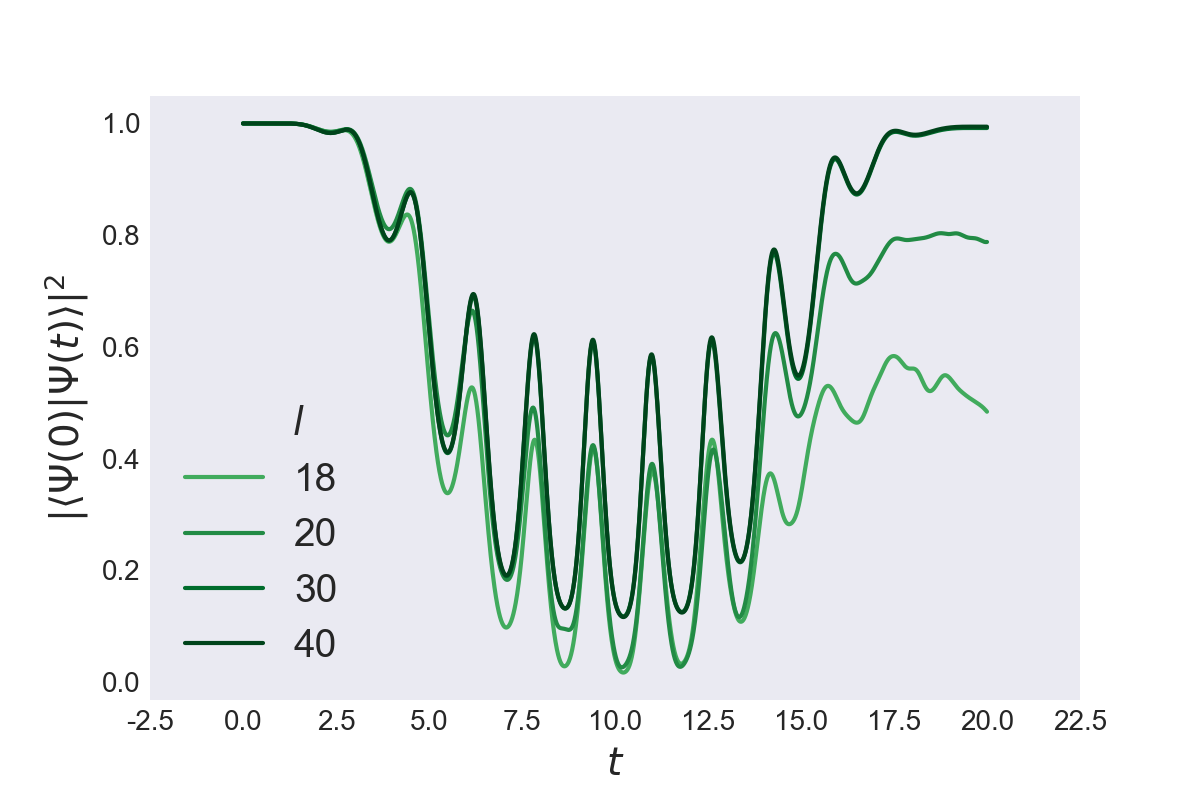
\includegraphics[width=\textwidth]{results/figures/1D/n=10overlap.png}
    \end{minipage}
    }
    \caption{Time-dependent energy (left) and ground state probability (right)
        of a one-dimensional harmonic oscillator with $\Omega=1 \text{ a.u.}$
        and $n=10$ electrons under the influence of a oscillating electric field 
        of frequency $\omega = 2 \Omega = 2 \text{ a.u.}$ and field strength
        $E_\text{max}=1 \text{ a.u.}$,
        for different number of spin-orbitals $l=\{18,20,30,40\}$.
    }
    \label{fig:1d_n10_qd}
\end{figure}

\begin{figure}[!h]
    \centering
    \makebox[\textwidth][c]{
    \begin{minipage}{0.6\textwidth}
        \centering
        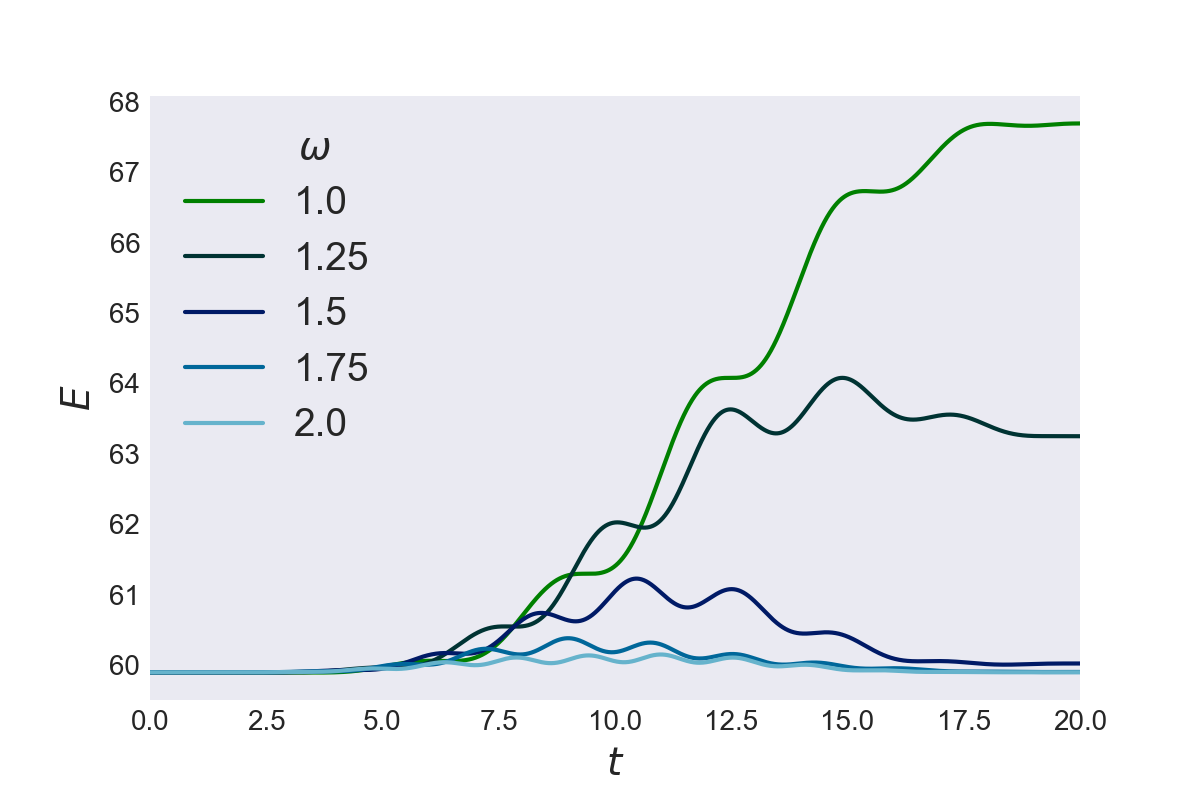
\includegraphics[width=\textwidth]{results/figures/1D/n10_resonance_energy.png}
    \end{minipage}\hfill 
    \begin{minipage}{0.6\textwidth}
        \centering 
        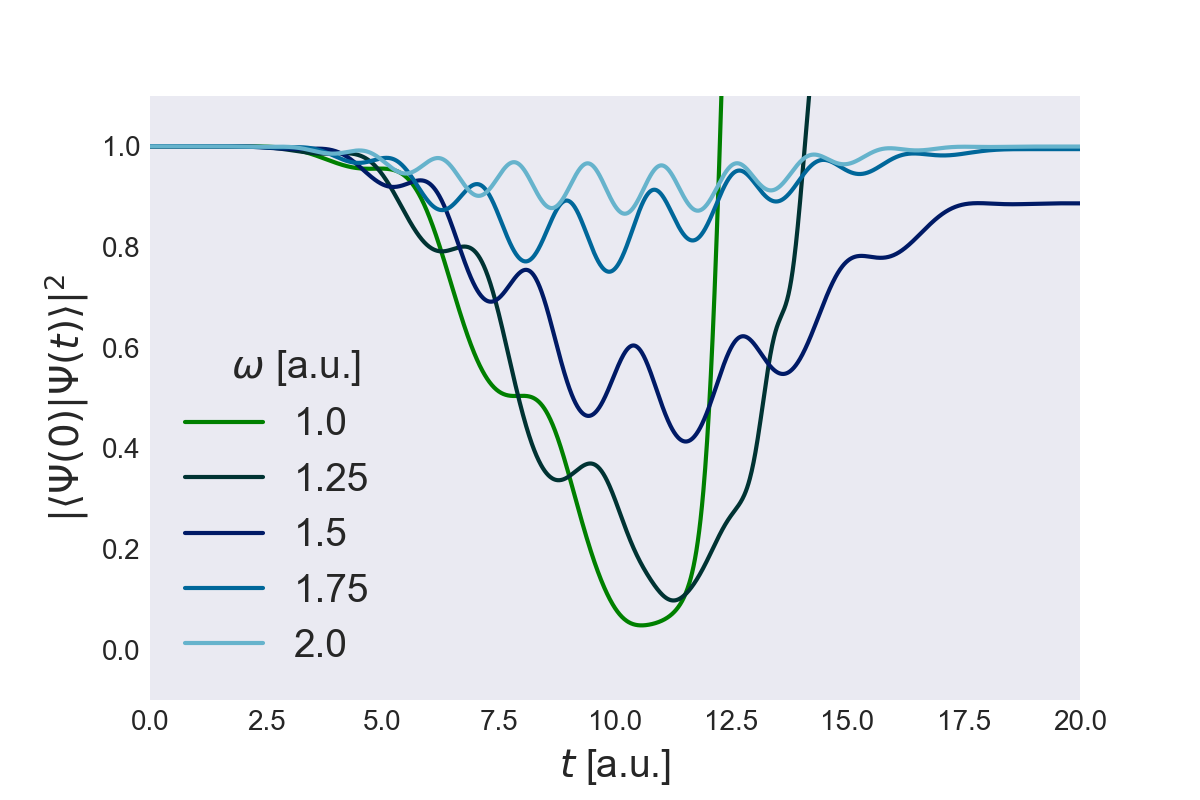
\includegraphics[width=\textwidth]{results/figures/1D/n10_resonance_overlap.png}
    \end{minipage}
    }
    \caption{Time-dependent energy (left) and ground state probability (right)
        of a one-dimensional harmonic oscillator with $\Omega=1 \text{ a.u.}$
        and $n=8$ electrons under the influence of a oscillating electric field 
        of different frequencies $\omega\in\{1.0, 1.25, 1.5, 1.75, 2.0\}$ in atomic units with 
        maximum field strength $E_\text{max}=0.25  \text{ a.u.}$ and $l=40$ 
        spin-orbitals.
    }
    \label{fig:1d_n10_qd_resonance}
\end{figure}

\vfill
\pagebreak

\subsection*{Twelve electrons}

\begin{figure}[!h]
    \centering
    \makebox[\textwidth][c]{
    \begin{minipage}{0.6\textwidth}
        \centering
        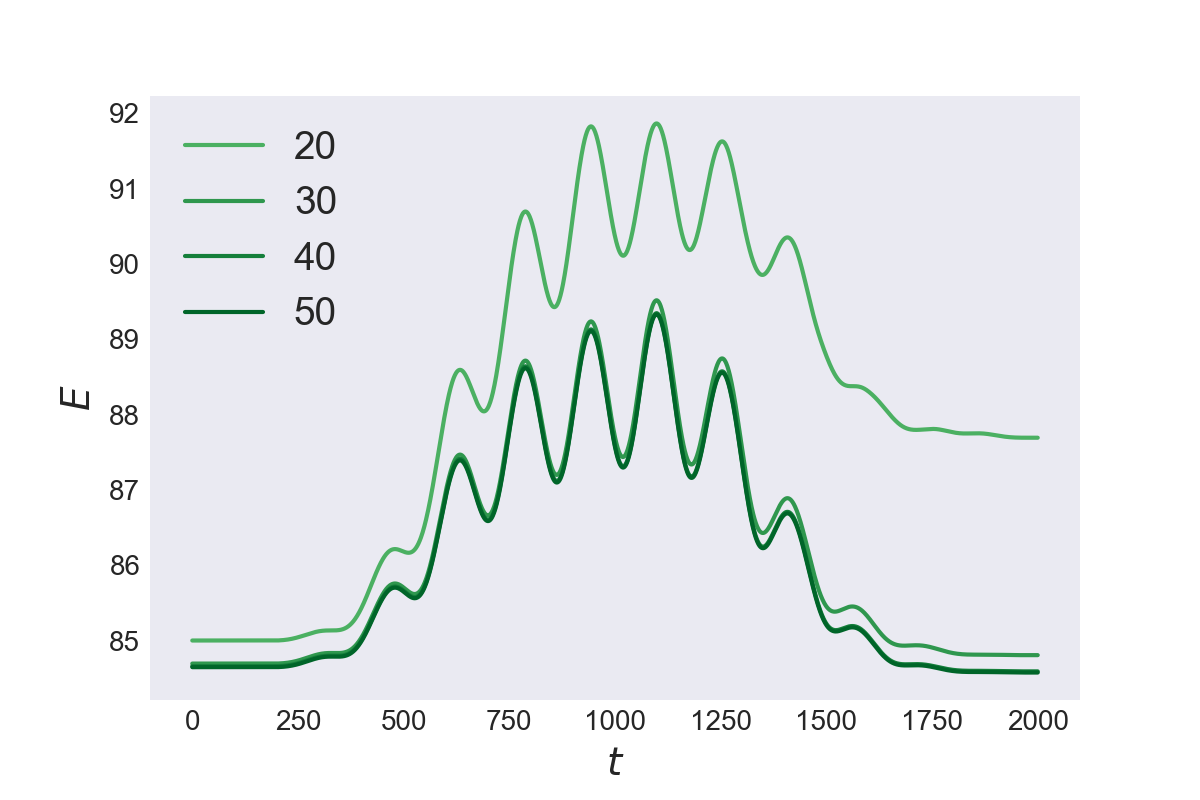
\includegraphics[width=\textwidth]{results/figures/1D/n=12energy.png}
    \end{minipage}\hfill 
    \begin{minipage}{0.6\textwidth}
        \centering 
        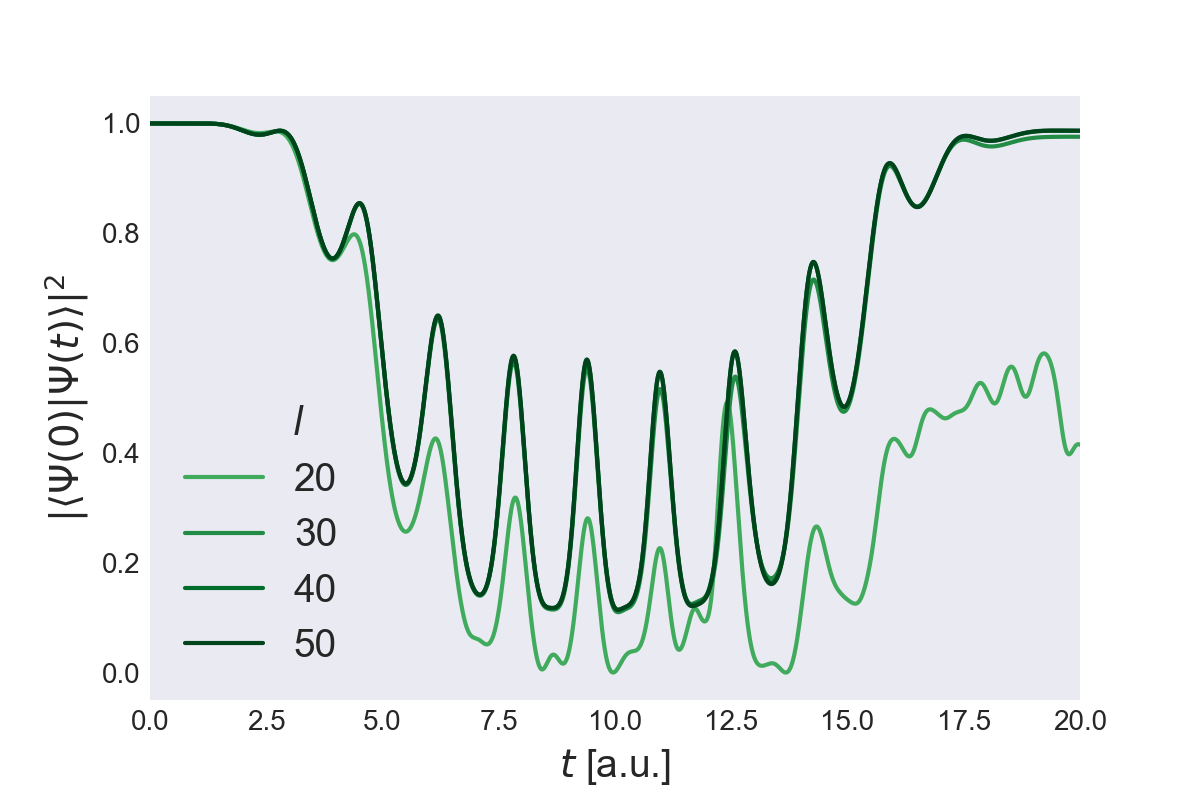
\includegraphics[width=\textwidth]{results/figures/1D/n=12overlap.png}
    \end{minipage}
    }
    \caption{Time-dependent energy (left) and ground state probability (right)
        of a one-dimensional harmonic oscillator with $\Omega=1 \text{ a.u.}$
        and $n=12$ electrons under the influence of a oscillating electric field 
        of frequency $\omega = 2 \Omega = 2 \text{ a.u.}$ and field strength
        $E_\text{max}=1 \text{ a.u.}$,
        for different number of spin-orbitals $l=\{20,30,40,50\}$.
    }
    \label{fig:1d_n12_qd}
\end{figure}

\vfill
\pagebreak


\section{Two Dimensions}
\label{app:supp_2d_qd_results}

The simulations presented here have been conducted with the Time-Dependent Coupled 
Cluster Singled Doubles (TDCCSD) method.

\subsection*{Two electrons}

\begin{figure}[!h]
    \centering
    \makebox[\textwidth][c]{
    \begin{minipage}{0.6\textwidth}
        \centering
        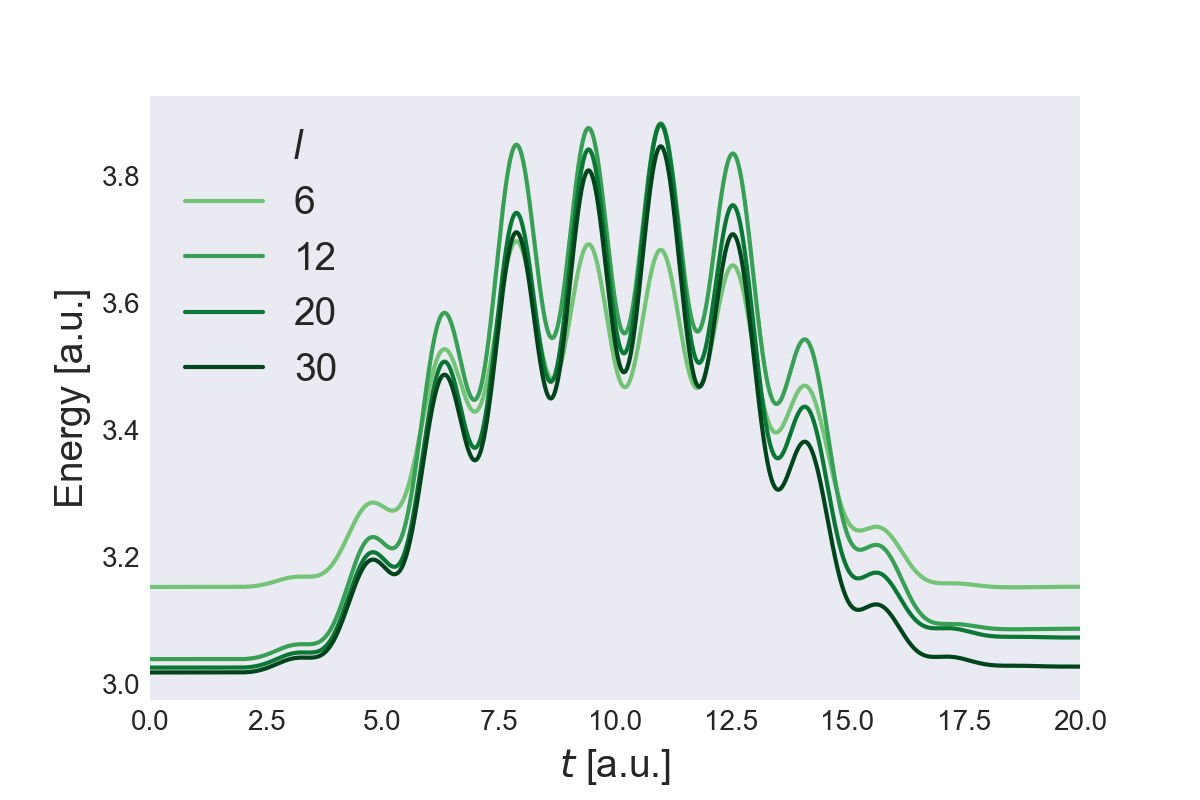
\includegraphics[width=\textwidth]{results/figures/2D/n2_energy.png}
    \end{minipage}\hfill 
    \begin{minipage}{0.6\textwidth}
        \centering 
        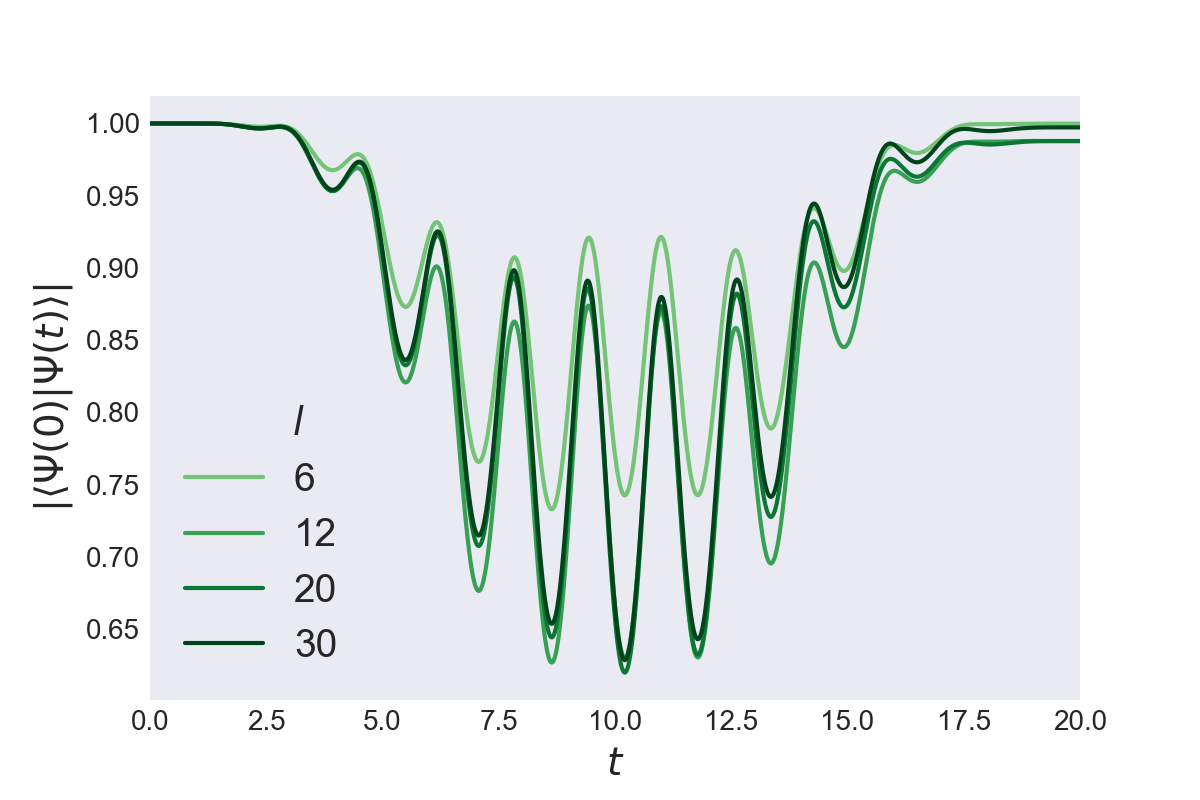
\includegraphics[width=\textwidth]{results/figures/2D/n2_overlap.png}
    \end{minipage}
    }
    \caption{Time-dependent energy (left) and ground state probability (right)
        of a two-dimensional harmonic oscillator with $\Omega=1 \text{ a.u.}$
        and $n=2$ electrons under the influence of a oscillating electric field 
        of frequency $\omega = 2 \Omega = 2 \text{ a.u.}$ and field strength
        $E_\text{max}=1 \text{ a.u.}$,
        for different number of spin-orbitals $l=\{6,12,20,30\}$.
    }
    \label{fig:2d_n2_qd}
\end{figure}


\subsection*{Six electrons}

\begin{figure}[!h]
    \centering
    \makebox[\textwidth][c]{
    \begin{minipage}{0.6\textwidth}
        \centering
        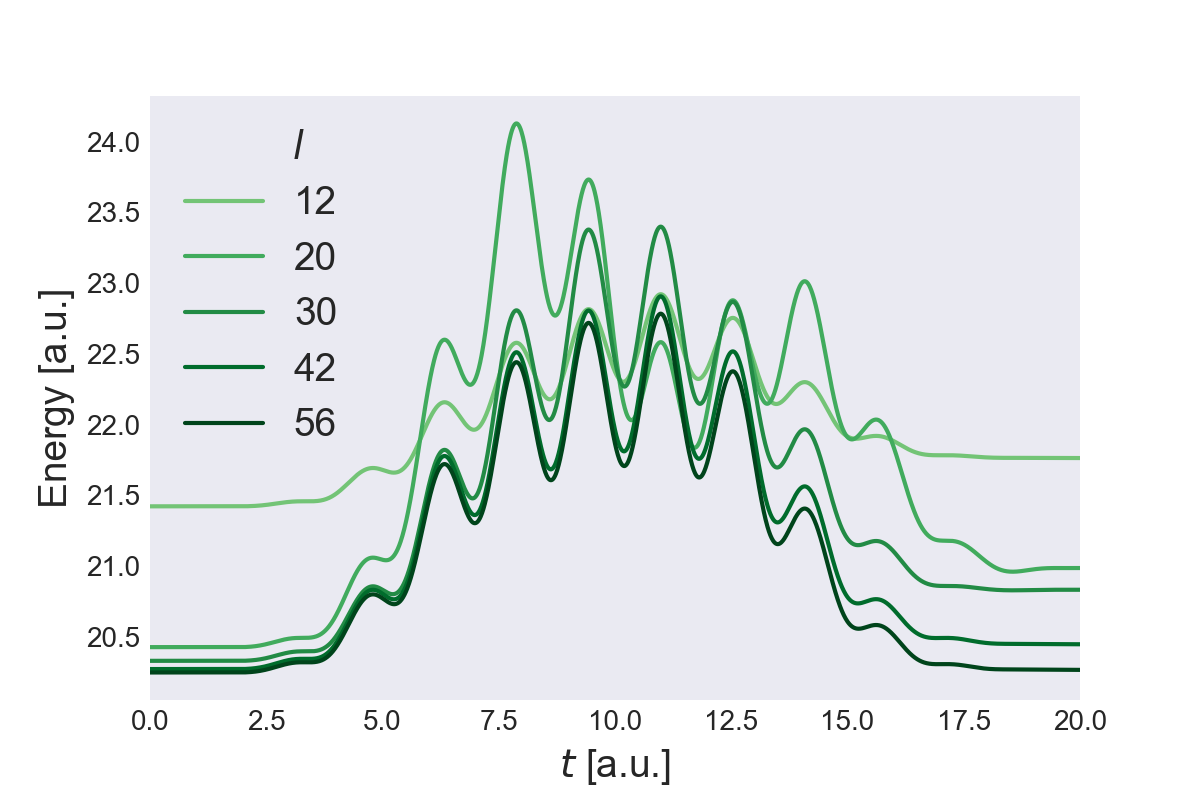
\includegraphics[width=\textwidth]{results/figures/2D/n6_energy.png}
    \end{minipage}\hfill 
    \begin{minipage}{0.6\textwidth}
        \centering 
        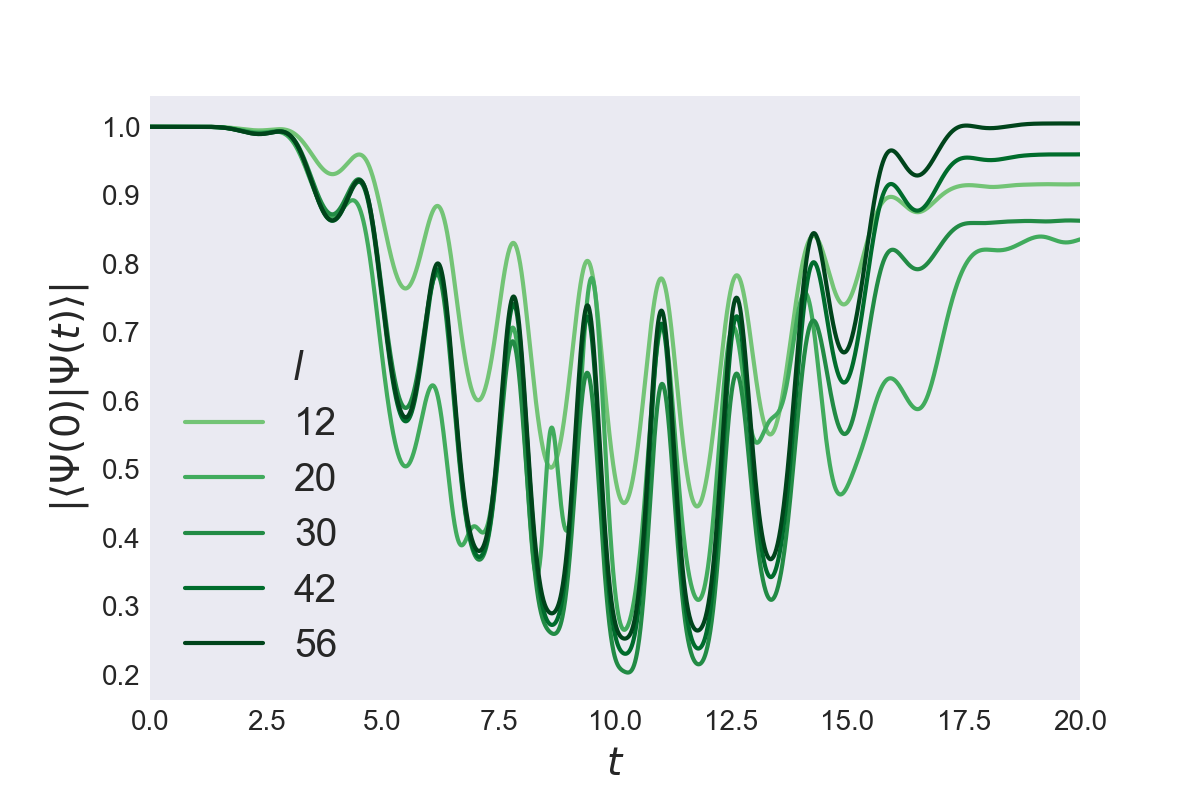
\includegraphics[width=\textwidth]{results/figures/2D/n6_overlap.png}
    \end{minipage}
    }
    \caption{Time-dependent energy (left) and ground state probability (right)
        of a two-dimensional harmonic oscillator with $\Omega=1 \text{ a.u.}$
        and $n=6$ electrons under the influence of a oscillating electric field 
        of frequency $\omega = 2 \Omega = 2 \text{ a.u.}$ and field strength
        $E_\text{max}=1 \text{ a.u.}$,
        for different number of spin-orbitals $l=\{12,20,30,42,56\}$.
    }
    \label{fig:2d_n6_qd}
\end{figure}

\vfill
\pagebreak

\section{Two Dimensions with Magnetic Field}
\label{app:b_field}

The simulations presented here have been conducted with the Orbital-Adaptive 
Time-Dependent Coupled Cluster Doubles (OATDCCD) method. 

\begin{figure}[!h]
    \centering
    \makebox[\textwidth][c]{
    \begin{minipage}{0.6\textwidth}
        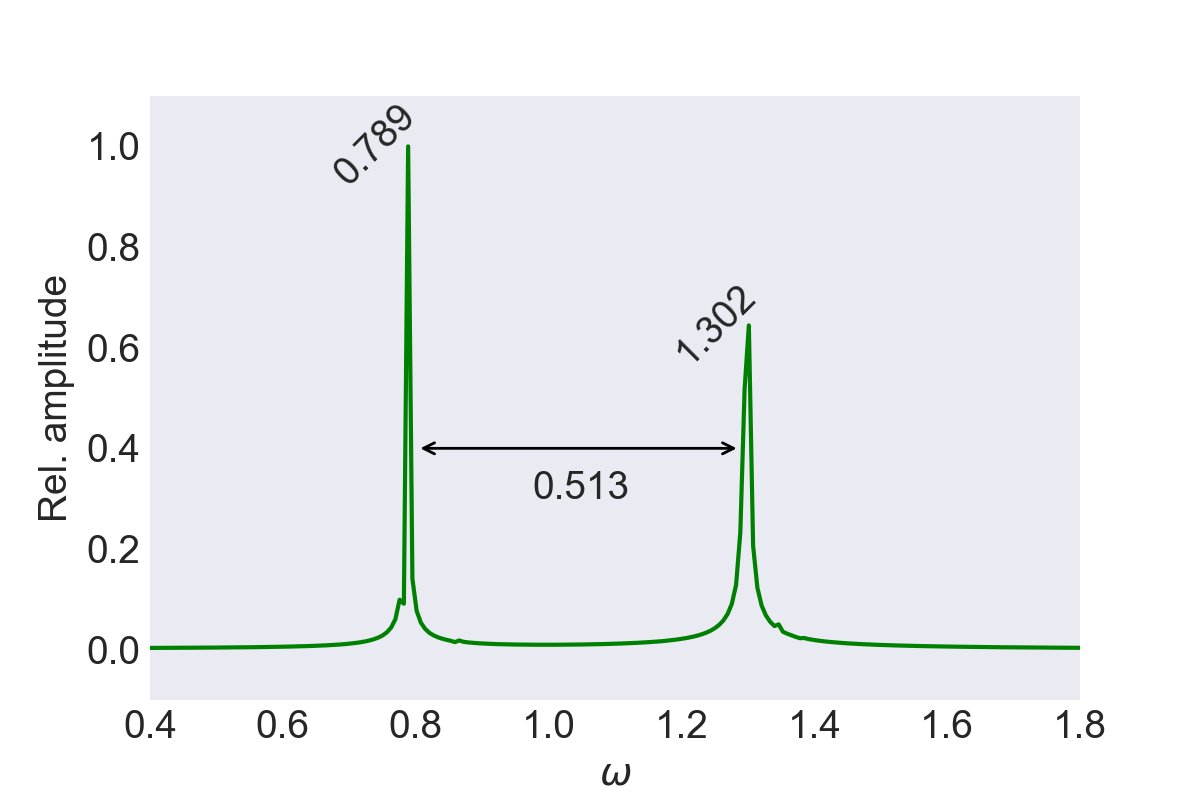
\includegraphics[clip=2em 0em 10em 0em, width=\textwidth]
        {results/figures/B_field/n=2/b_spectrum_omc050.png}
    \end{minipage}\hfill 
    \begin{minipage}{0.6\textwidth}
        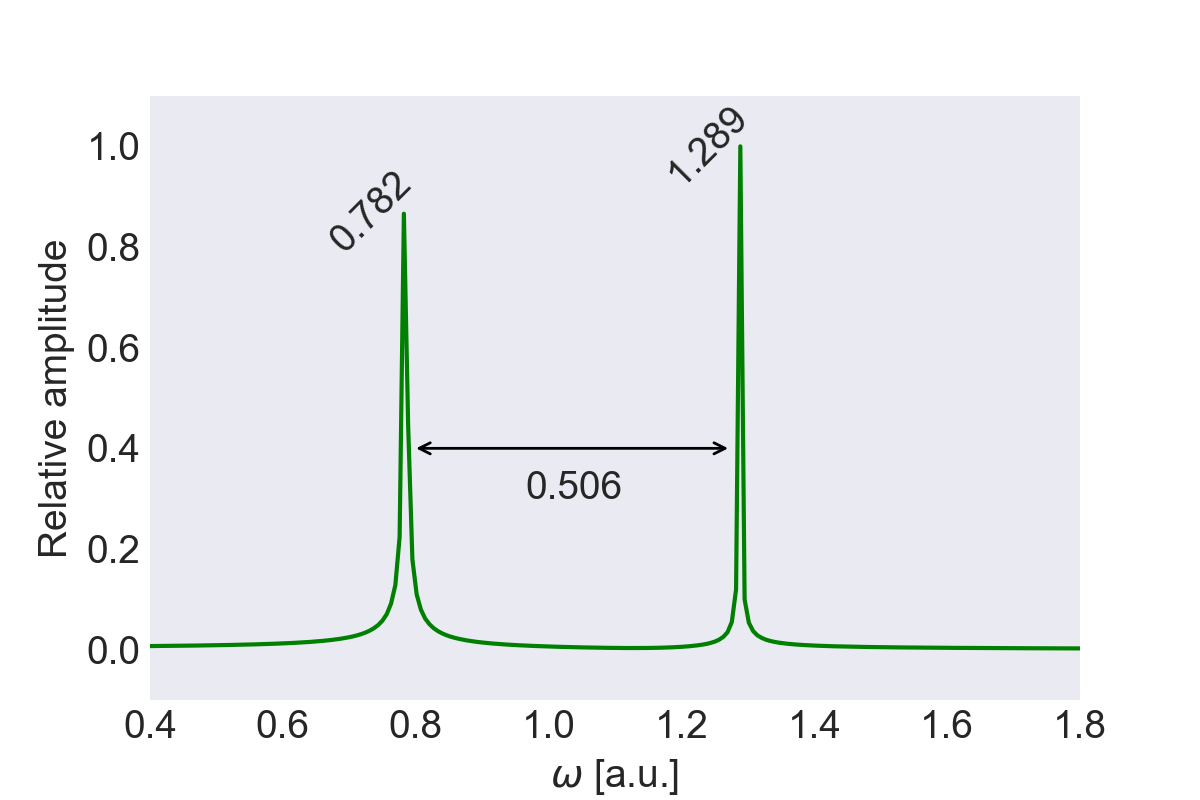
\includegraphics[clip=0em 0em 10em 0em, width=\textwidth]
        {results/figures/B_field/n=4/b_spectrum_n=4_omc=050.png}
    \end{minipage}
    }
    \caption{Dipole spectrum of a quantum dot with $n=2$ (left), and $n=4$ electron 
    subjected to a magnetic field with Larmor frequency $\omega_c=0.50 \text{ a.u.}$.
    Both systems have base oscillator frequency $\omega_0=1 \text{ a.u.}$ and 
    have been excited with an oscillating field with frequency $\omega = 1 \text{ a.u.}$
    and intensity $E_\text{max} = 0.1 \text{a.u.}$. The oscillating field had a period of 
    $t_d = 6\pi/\omega \text{ a.u.}$ and the system was developed in time for a total 
    of $T = 1000 \text{ a.u.}$.}
    \label{fig:b_omc050}
\end{figure}

\begin{figure}[!h]
    \centering
    \makebox[\textwidth][c]{
    \begin{minipage}{0.6\textwidth}
        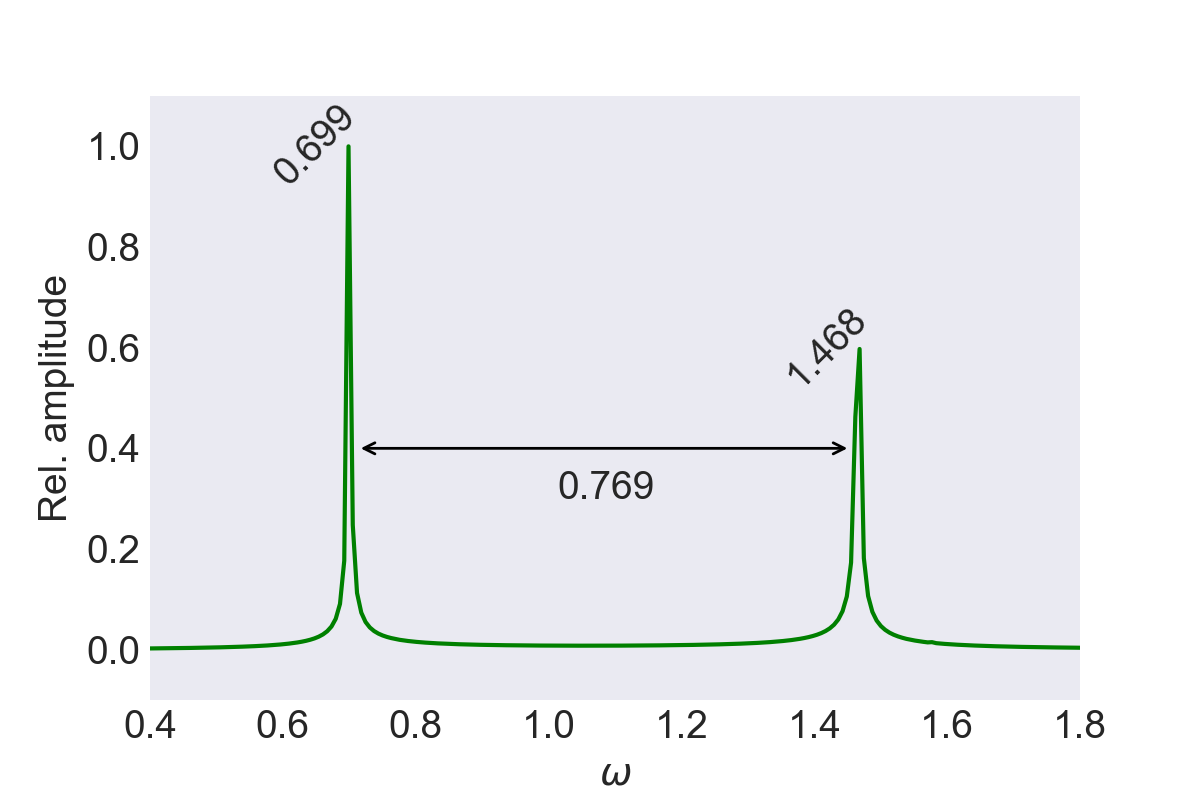
\includegraphics[clip=2em 0em 10em 0em, width=\textwidth]
        {results/figures/B_field/n=2/b_spectrum_omc075.png}
    \end{minipage}\hfill 
    \begin{minipage}{0.6\textwidth}
        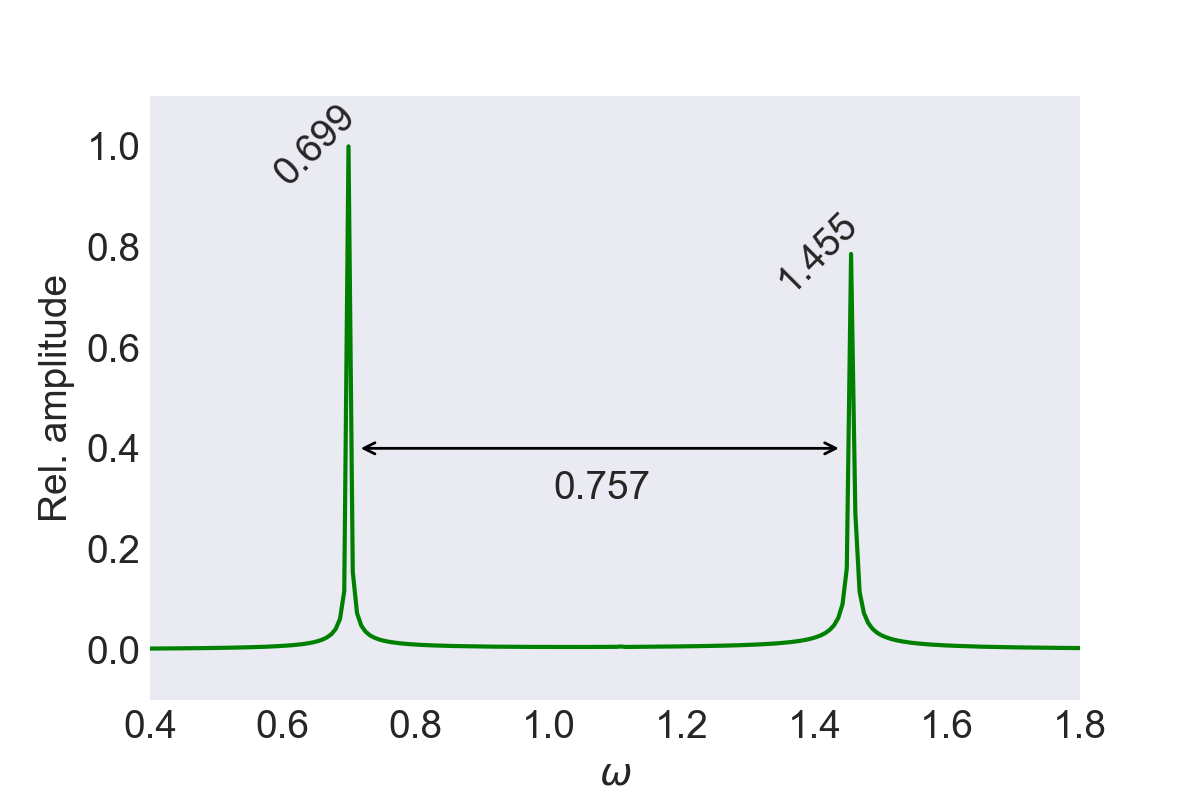
\includegraphics[clip=0em 0em 10em 0em, width=\textwidth]
        {results/figures/B_field/n=4/b_spectrum_n=4_omc=075.png}
    \end{minipage}
    }
    \caption{Dipole spectrum of a quantum dot with $n=2$ (left), and $n=4$ electron 
    subjected to a magnetic field with Larmor frequency $\omega_c=0.75 \text{ a.u.}$.
    Both systems have base oscillator frequency $\omega_0=1 \text{ a.u.}$ and 
    have been excited with an oscillating field with frequency $\omega = 1 \text{ a.u.}$
    and intensity $E_\text{max} = 0.1 \text{a.u.}$. The oscillating field had a period of 
    $t_d = 6\pi/\omega \text{ a.u.}$ and the system was developed in time for a total 
    of $T = 1000 \text{ a.u.}$.}
    \label{fig:b_omc075}
\end{figure}

\begin{figure}[!h]
    \centering
    \makebox[\textwidth][c]{
    \begin{minipage}{0.6\textwidth}
        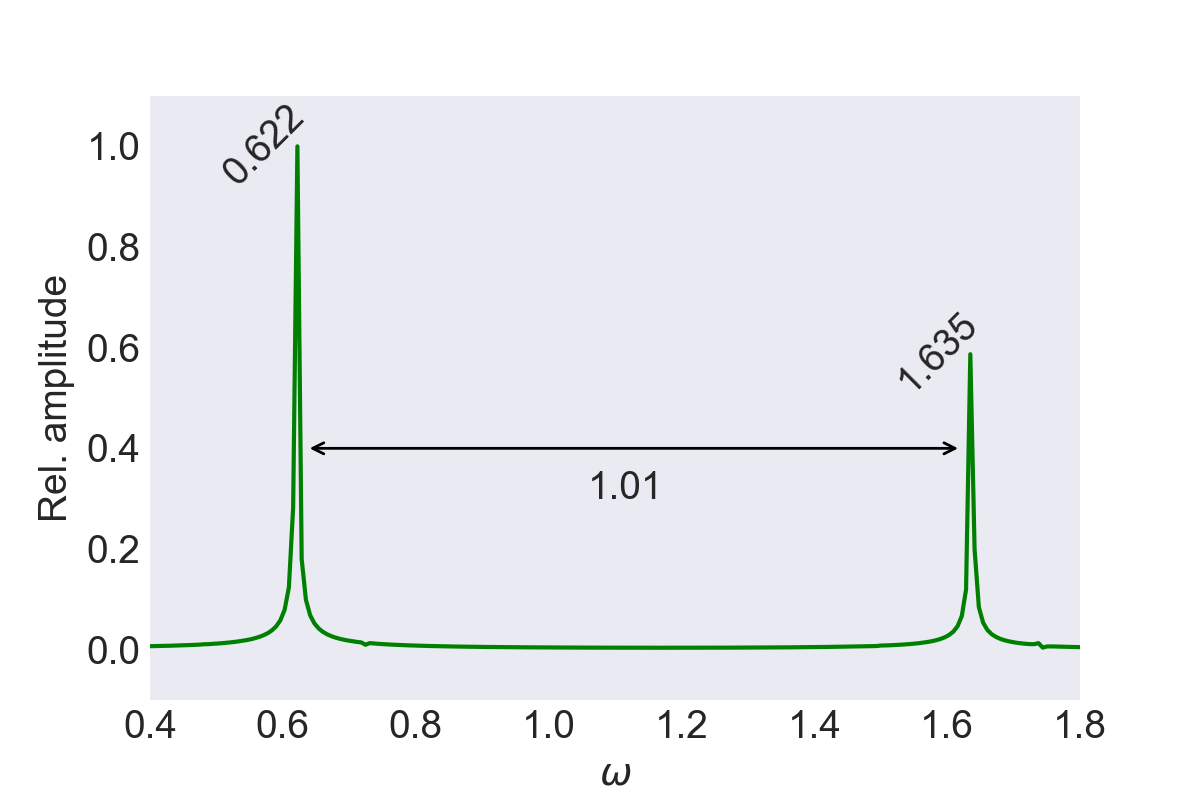
\includegraphics[clip=2em 0em 10em 0em, width=\textwidth]
        {results/figures/B_field/n=2/b_spectrum_omc100.png}
    \end{minipage}\hfill 
    \begin{minipage}{0.6\textwidth}
        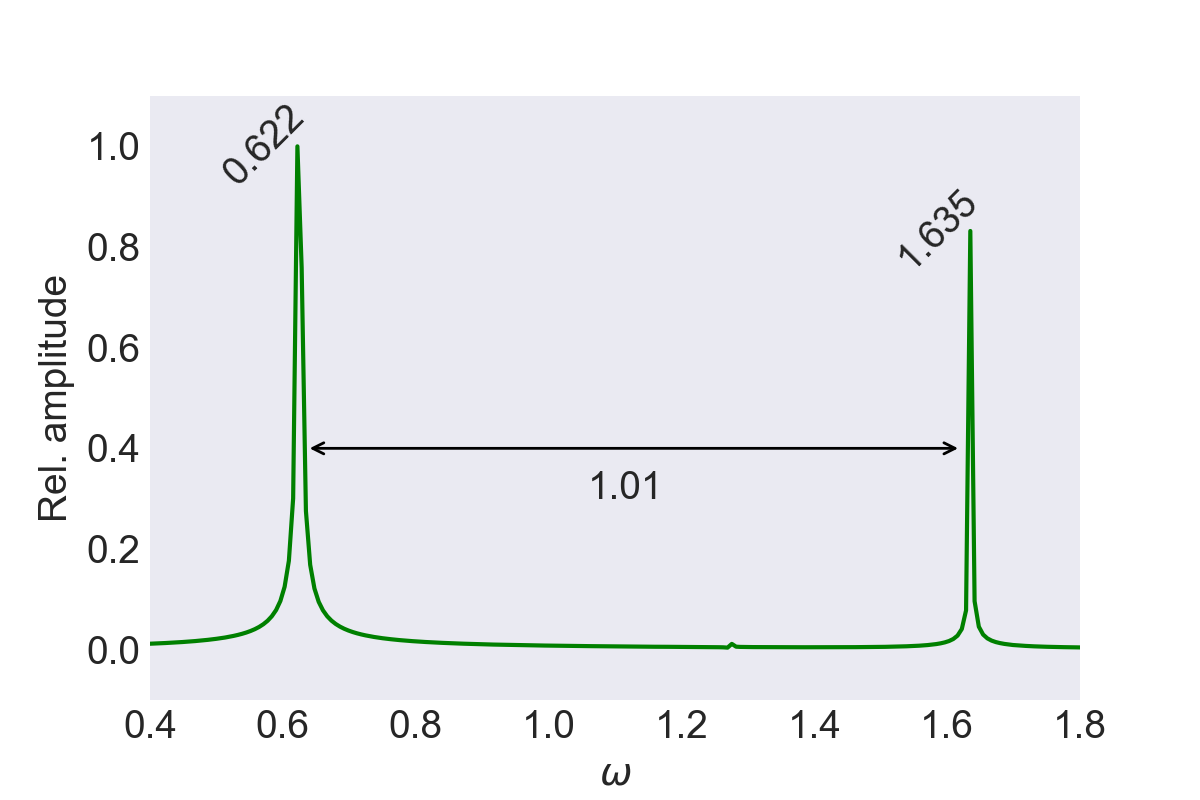
\includegraphics[clip=0em 0em 10em 0em, width=\textwidth]
        {results/figures/B_field/n=4/b_spectrum_n=4_omc=100.png}
    \end{minipage}
    }
    \caption{Dipole spectrum of a quantum dot with $n=2$ (left), and $n=4$ electron 
    subjected to a magnetic field with Larmor frequency $\omega_c=1.0 \text{ a.u.}$.
    Both systems have base oscillator frequency $\omega_0=1 \text{ a.u.}$ and 
    have been excited with an oscillating field with frequency $\omega = 1 \text{ a.u.}$
    and intensity $E_\text{max} = 0.1 \text{a.u.}$. The oscillating field had a period of 
    $t_d = 6\pi/\omega \text{ a.u.}$ and the system was developed in time for a total 
    of $T = 1000 \text{ a.u.}$.}
    \label{fig:b_omc100}
\end{figure}

\vfill
\pagebreak

\clearemptydoublepage